\documentclass[]{tufte-book}

% ams
\usepackage{amssymb,amsmath}

\usepackage{ifxetex,ifluatex}
\usepackage{fixltx2e} % provides \textsubscript
\ifnum 0\ifxetex 1\fi\ifluatex 1\fi=0 % if pdftex
  \usepackage[T1]{fontenc}
  \usepackage[utf8]{inputenc}
\else % if luatex or xelatex
  \makeatletter
  \@ifpackageloaded{fontspec}{}{\usepackage{fontspec}}
  \makeatother
  \defaultfontfeatures{Ligatures=TeX,Scale=MatchLowercase}
  \makeatletter
  \@ifpackageloaded{soul}{
     \renewcommand\allcapsspacing[1]{{\addfontfeature{LetterSpace=15}#1}}
     \renewcommand\smallcapsspacing[1]{{\addfontfeature{LetterSpace=10}#1}}
   }{}
  \makeatother

\fi

% graphix
\usepackage{graphicx}
\setkeys{Gin}{width=\linewidth,totalheight=\textheight,keepaspectratio}

% booktabs
\usepackage{booktabs}

% url
\usepackage{url}

% hyperref
\usepackage{hyperref}

% units.
\usepackage{units}


\setcounter{secnumdepth}{-1}

% citations
\usepackage{natbib}
\bibliographystyle{plainnat}


% pandoc syntax highlighting

% table with pandoc

% multiplecol
\usepackage{multicol}

% strikeout
\usepackage[normalem]{ulem}

% morefloats
\usepackage{morefloats}


% tightlist macro required by pandoc >= 1.14
\providecommand{\tightlist}{%
  \setlength{\itemsep}{0pt}\setlength{\parskip}{0pt}}

% title / author / date
\title[Reynolds and Currie]{Transit Supply Index scores on the days of
the 2016 and 2021 censuses: using Statistical Area Level 1 (SA1) 2016
boundaries}
\author{James Reynolds and Graham Currie}
\date{2023-08-22}

\usepackage{fancyhdr}
\pagestyle{fancy}
\fancyhead[LE]{\textsc{Leveraging GTFS: \leftmark; \rightmark}}
\fancyhead[RO]{\textsc{Reynolds and Currie}}
\fancyfoot[LE]{\thepage \hspace{1em} \textsc{Department of Civil Engineering, Monash University}}
\fancyfoot[RO]{\textsc{Public Transport Research Group, Institute of Transport Studies} \hspace{1em} \thepage}
\usepackage{titling}
\pretitle{\begin{center} 
\includegraphics[width=2in,height=2in]{ptrg-logo-s.png}\LARGE\\}
\posttitle{\end{center}}
\usepackage{booktabs}
\usepackage{longtable}
\usepackage{array}
\usepackage{multirow}
\usepackage{wrapfig}
\usepackage{float}
\usepackage{colortbl}
\usepackage{pdflscape}
\usepackage{tabu}
\usepackage{threeparttable}
\usepackage{threeparttablex}
\usepackage[normalem]{ulem}
\usepackage{makecell}
\usepackage{xcolor}

\begin{document}

\maketitle




\hypertarget{introduction}{%
\chapter{Introduction}\label{introduction}}

Previous research by \citet{currie2007identifying} developed a transit
Supply Index (SI), based on calculating the number of transit arrivals
at stops within an area of interest, adjusted to account for the typical
walk-access catchment for each stop. This document reports the
development of R code to calculate the Supply Index of
\citet{currie2007identifying} directly from GTFS data. The code is used
to output SI scores for the day of the 2016 census and the day of the
2021 census for each of the Australian Bureau of Statistics (ABS) 2016
Statistical Area Level 1 (SA1) zones in Victoria. These scores have been
requested by Maryam Jafari as an input to her PhD project.

This rest of this document is structured as follows: the next section
discusses the research context of transit metrics and the the Supply
Index. In the third section the methodology for the code development is
outlined, including discussion of the case study GTFS for Victoria,
Australia, that was used to test and verify the code output. In the
fourth section results are presented, starting with verification of the
code output through hand-calculation of SI scores for Statistical Area 1
(SA1) areas in the Victorian Alps and Talbot. SI scores for SA1s across
Greater Melbourne and Victoria are also presented. Mode-by-mode SI
scores are also explored, followed by an examination of needs-gaps
across the ABS Index for Relative Socio-Economic Advantage/Disadvantage
(IRSAD) scores, ranks and population levels. The document then closes
with a brief discussion and conclusion section.

\hypertarget{research-context}{%
\chapter{Research context}\label{research-context}}

\hypertarget{the-suppy-index}{%
\section{The Suppy Index}\label{the-suppy-index}}

\begin{marginfigure}
\begin{equation}
\label{eq:supply_index}
SI_{area, time} = \sum{\frac{Area_{Bn}}{Area_{area}}*SL_{n, time}}
\end{equation}
\end{marginfigure}

Equation \ref{eq:supply_index}\footnote{In Equation
  \ref{eq:supply_index} \(SI_{area, time}\) is the Supply Index for the
  area of interest and a given period of time. \(Area_{Bn}\) is the
  buffer area for each stop (n) within the area of interest. In
  \citet{currie2007identifying} this was based on a radius of 400 metres
  for bus and tram stops, and 800 metres for railway stations.
  \(Area_area\) is the area of the area of interest, and \(SL_{n,time}\)
  is the number of transit arrivals for each stop for a given time
  period.} shows the Supply Index\footnote{Minor adjustments have been
  made to generalise the equation, as \citet{currie2007identifying}
  focused on the context of Melbourne's Census Collection Districts
  (CCD) and calculations based on a week of transit service.}. An
advantage of the Supply Index is that it is a relatively simple number
to calculate, understand and explain. It describes the number of transit
arrivals at stops within an area of interest and time frame, multiplied
by a factor accounting for the proportion of the area of interest that
is within typical walking distance of each stop. Hence, more services,
more stops and higher frequencies would all result in an increase in
Supply Index score. The Supply Index does not incorporate further
aspects, such as service span, off-peak share of service or service
speed, which are a feature of the TQCSM. However, including such metrics
may increase the complexity of calculating and describing the index to
non-transit specialists. Such simplicity is also helped by the way that
the Index is additive, in that \(SI_{area, time}\) scores can be
aggregated to calculate an overall score across multiple time periods or
for a region encompassing multiple areas of interest.

\citet{currie2007identifying} calculated the \(SI_{area, time}\) for
various Census Collection Districts (CCDs)\footnote{CCDs predate the
  introduction of Statistical Areas 1, 2, 3, and 4 (SA1, SA2, SA3, SA4),
  and other geographical divisions currently used by the Australian
  Bureau of Statistics (ABS), which may be more familiar to readers.} in
Melbourne using a timetable database provided by the Victorian Public
Transport Authority (PTA). This predated the widespread availability of
GTFS data. A question, therefore, is how to calculate the SI using GTFS
data so that \(SI_{area, time}\) scores can be calculated and compared
for any area of interest where transit service information is available
in that format.

\hypertarget{transport-needs-indexes}{%
\section{Transport Needs Index(es)}\label{transport-needs-indexes}}

\citet{currie2007identifying} also developed a Transport Needs Index
based around population, transport and employment data. This was
combined with the ABS' Index for Relative Socio-Economic
Advantage/Disadvantage (IRSAD) to produce a combine index addressing
social and transport needs Later in this document a similar needs-gap
analysis is presented for Victorian SA1s. However, in the needs-gap
analysis here only the IRSAD scores and population data are reported.
Calculating the combined Transport Needs index as per
\citet{currie2007identifying} may be a direction for future research.

Various analysis tools are available that make use of GTFS data,
including the tidytransit package \citep{R-tidytransit} for the R
statistical programming language \citep{R-base}.
\citet{tidytransit_departure_timetable} provides code to calculate a
departure timetable from a GTFS feed, and this was adapted to calculate
arrivals at a stop and the SL\textsubscript{Bn} term in the
\citet{currie2007identifying} SI equation.

The gtfstools R package \citep{R-gtfstools} was used to split input GTFS
feeds by mode to facilitate the buffer zone calculation. Buffer zones of
400 metres for bus and Light Rail Transit (LRT) services and 800 metres
for heavy rail were adopted, as per
\citet{currie2007identifying}\footnote{There is an extended mode
  definition that includes modes beyond the 10 in the GTFS standard
  \citep{filter_GTFS_by_mode}, but these are not dealt with by the
  gtfstools package. Further research may seek to extend this such that
  other modes can be included, but for the purposes of this study the
  coded buffer zone was set at 400 metres for cable trams, aerial lifts
  such a gondolas and trolleybuses, and at 800 metres for ferries,
  funiculars and monorails.}.

Where transit stops are located close to boundaries their catchment
areas may fall into multiple areas of interest. The sp package
\citep{R-sf} provides tools for manipulating geographic data and shape
files in R. This was used to calculate the proportion of each stop's
catchment area that falls into each geographical area of
interest\footnote{GTFS files define stop locations based on latitude and
  longitude \citep{GTFS}, whereas the Area\textsubscript{Bn} calculation
  needs to be provided in the same units as the Area\textsubscript{area}
  variable, necessitating the use of a geographic transform as part of
  the code.}.

The SI\textsubscript{area} term in the SI equation was calculated on a
mode-by-mode and stop-by-stop basis, by first determining the amount of
the catchment area (Area\textsubscript{Bn}) that falls into each
geographical area of interest for the stop in question. This is then
combined with the area for each geographical area of interest
(Area\textsubscript{area}) and the number of stop arrivals
(SL\textsubscript{Bn}) to calculate the contribution to the SI scores
made by just that single stop for every area of interest. These are then
added to a cumulative total field for each area of interest, and the
calculations are repeated until all stops and modes in the GTFS file
have been included.

\hypertarget{case-research-approach}{%
\section{Case research approach}\label{case-research-approach}}

To test the developed code and output results analysis was generated for
SA1 zones within two case study areas: Clayton (SA2) and Melbourne City
(SA3). Results were processed using the ggmaps \citep{R-ggmap}, ggplot
\citep{R-ggplot2}, ggstatsplot \citep{R-ggstatsplot} and kable
\citep{R-kableExtra, R-knitr} packages, with data processing leveraging
the tidyverse approach \citep{R-tidyverse}.

\hypertarget{victoria-australia}{%
\subsection{Victoria, Australia}\label{victoria-australia}}

Victoria is the southern-most state on the Australian mainland. The
state capital is in Melbourne, which has a similar metropolitan area to
of Paris or London\footnote{Greater Melbourne is the term used to
  describe the larger metropolitan area, encompassing 30 LGAs. The City
  of Melbourne LGA covers only a small portion of the inner city.}.
However, with only around 5 million people Melbourne has about one-third
of the population density. It has an inner Central Business District
(CBD) with apartments, commercial skyscrapers and extensive sporting
facilities nearby; surrounded by low-density, predominately
single-family-housing-dominated, inner, middle and outer suburbs.

There are train and tram networks radiating from the CBD, but for most
of the suburban areas the reality is that transit is provided by
circuitious bus routes that are mostly used by those who cannot
otherwise drive. An extensive freeway (and tollway) network provides
connections across the Greater Melbourne area, further around Port
Phillip Bay to Geelong (south-west) and the Mornington Penninsula
(south-east) as well as to regional centres elsewhere in Victoria. There
is a state-wide regional train and bus network (VLine), which also
provides connections into South Australia, New South Wales and the
Australian Capital Territory (Canberra) and local bus services in many
regional towns and cities. However, accessibility to most of the city
and state tends to be car-dominated. The Overland train service to
Adelaide and the XPT to Sydney are provided seperately to VLine
services. Victoria's GTFS feed is published by Public Transport Victoria
(PTV)\footnote{There are over 400 historical releases of the available
  on the transitfeeds.com website, with the first dating from March 2015
  \citep{transitfeeds_victoria:2023aa}.}.

The developed code has been separately tested using SA1- and LGA-level
areas of interest, including hand verification of some example SA1
areas\footnote{This testing is reported in the main branch of the
  project on GitHub. This document is instead specific to the
  calculation of the SI scores for the 2016 SA1 boundaries.}. For the
results reported here output was obtained for SA1-level areas using GTFS
files from August 2016 and 2021, running for just the day of the census
in each year. The Australian census is undertaken in early August every
5 years. GTFS feeds were therefore selected for the first week of August
of each year, with code output produced for only the day of the census
itself\footnote{It takes about a day of processing time to run the code
  for all of the stops in Victoria for a single `day' of service. Hence,
  only the census days (rather than weeks) were analysed to speed
  development.}. Minor corrections were made to the GTFS files to remove
duplicate stop\_ids\footnote{These involved minor discrepancies in
  either the stop name, latitude or longitude.}.

The Australian Bureau of Statistics (ABS) provides a range of shape
files and other resources. This study made use of the absmapsdata R
package \citep{R-absmapsdata} to access the 2016 SA1 boundaries for
Victoria. The EPSG:28355 transform \citep{EPSG_28355} was used to shift
longitude and latitude into metres, as per the Geocentric Datum of
Australia 1994 (GDA95 / MGA zone 55) coordinates.

The ABS provides IRSAD datasets for SA1 in excel format. Data for 2016
and 2021 was included in this study\footnote{The IRSAD scores for 2021
  appear to only be available for the SA12021 boundaries. A
  correspondance file was used to match the SA12021 to SA12016
  boundaries, but it was not possible to factor the scores.}. Scores for
2021 are shown in Figures \ref{fig:Victoria_IRSAD_load_2016} and
\ref{fig:Victoria_IRSAD_load_2021} for the Melbourne City and Clayton
case study areas.

\begin{figure*}
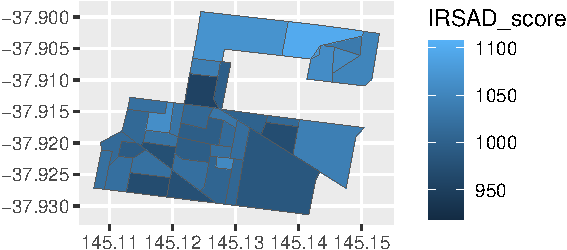
\includegraphics[width=0.5\linewidth]{Reynolds_Currie_2024_transit_supply_index_GTFS_files/figure-latex/Victoria_IRSAD_load_2021-1} 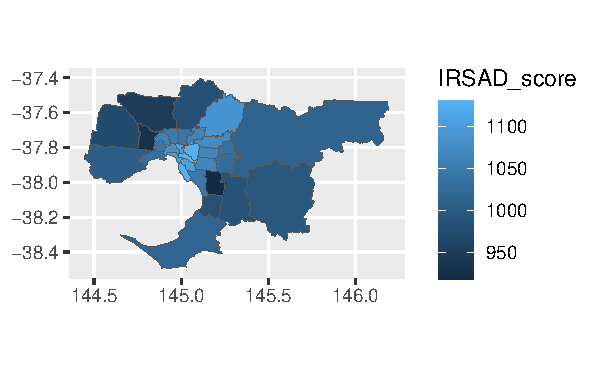
\includegraphics[width=0.5\linewidth]{Reynolds_Currie_2024_transit_supply_index_GTFS_files/figure-latex/Victoria_IRSAD_load_2021-2} \caption[2021 IRSAD score for SA1s]{2021 IRSAD score for SA1s: within the Clayton SA2 zone (left) and within the Melbourne City SA3 zone (right)}\label{fig:Victoria_IRSAD_load_2021}
\end{figure*}

The ISRAD scores appear to meet expectations. In Clayton there is no
score reported for the Monash University campus\footnote{Likely due to
  low resident population.}. Higher scores are reported for SA1s to the
north-east of Clayton, in the Notting Hill area. For the Melbourne City
SA3 zone, there are no ISRAD scores reported for the various
parks\footnote{Royal Park to the north, Fitzroy Gardens and the sporting
  district to the east and south east, and the SA1 with the Docklands
  stadium in it.}. Areas with lower IRSAD scores are located in parts of
North Melbourne and in the north-east \footnote{Lygon Street and
  Nicholson Street areas.}, which meets expectations.

\hypertarget{results}{%
\chapter{Results}\label{results}}

The following subsections discuss the results of running the code for
all of Victoria for 2016 and 2021, and the looks in detail at the two
selected cases (Clayton and Melbourne City) as a validation of the
results.

\hypertarget{supply-index-results-for-all-of-victoria}{%
\section{Supply Index results for all of
Victoria}\label{supply-index-results-for-all-of-victoria}}

Four files are included with this document\footnote{And in the `results'
  subdirectory of the SA12016 branch in the github repository.}. These
include the total 2016 and 2021 SI scores for each SA12016
zone\footnote{Victoria\_2016\_SA\_SA2016\_160809.csv and
  Victoria\_2021\_SI\_SA12016\_210810.csv}, and the SI scores by
mode\footnote{Victoria\_2016\_SI\_df\_by\_mode\ldots etc.}.

Figure \ref{fig:Victoria_SI_2021} show the \(SI_{LGA2021, 10/8/21}\)
values for Victoria (left) and Greater Melbourne (right).

The next sections show results for SA1 zones within Clayton and within
Greater Melbourne, so as to provide some context for the results and as
a cross-check.

\hypertarget{sa1s-within-the-clayton-sa2-zone}{%
\section{SA1s within the Clayton SA2
zone}\label{sa1s-within-the-clayton-sa2-zone}}

\begin{figure*}
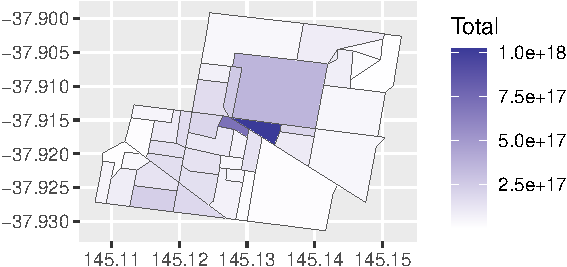
\includegraphics[width=0.5\linewidth]{Reynolds_Currie_2024_transit_supply_index_GTFS_files/figure-latex/Clayton_SI_2016_and_2021_maps-1} 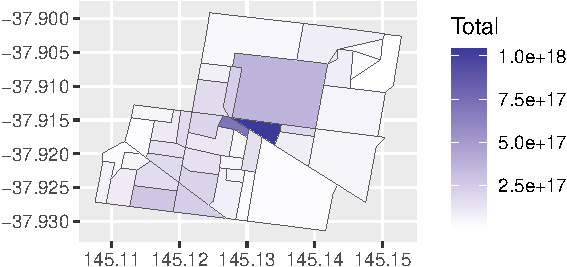
\includegraphics[width=0.5\linewidth]{Reynolds_Currie_2024_transit_supply_index_GTFS_files/figure-latex/Clayton_SI_2016_and_2021_maps-2} \caption[SA1s witihn the Clayton SA2 zone]{SA1s witihn the Clayton SA2 zone: SI for 2016 (left) and 2021 (right) census days}\label{fig:Clayton_SI_2016_and_2021_maps}
\end{figure*}

Figure \ref{fig:Clayton_SI_2016_and_2021_maps} shows SI scores for

\hypertarget{sa1s-within-the-melbourne-city-sa3-zone}{%
\section{SA1s within the Melbourne City SA3
zone}\label{sa1s-within-the-melbourne-city-sa3-zone}}

\hypertarget{examining-sa1s-across-all-of-greater-melbourne-and-all-of-victoria}{%
\section{Examining SA1s across all of Greater Melbourne and all of
Victoria}\label{examining-sa1s-across-all-of-greater-melbourne-and-all-of-victoria}}

\renewcommand\refname{References}
\bibliography{packages.bib,References.bib}



\end{document}
